\subsection{Producing lower bounds}
\label{sec:lb}


By definition of the CJSR, the asymptotic growth rate of the norm of the product of any $\G$-admissible (or $\G^\Tr $-admissible) sequence of matrices gives a lower bound on the CJSR.
In particular the sequence produced by Algorithm~\ref{algo:prodl} provides a lower bound on the CJSR.

If there are two integers $\bar{k},k$ such that the sequence after $\bar{k}$ is periodic of period $k$,
the asymptotic growth rate of the norm is equal to the $k$th root of the spectral radius of the product of the matrices of one period.
This is due to the Gelfand's formula $\rho(A) = \lim_{k \to \infty} \|A^k\|^{1/k}$.
From the same identity,
we see that the spectral radius of the product of the matrices of one $\G$-admissible cycle gives a lower bound on the CJSR.



To find lower bounds for the CJSR,
one could generate all the cycles of length smaller than some maximum length
and compute the spectral radius for all of them.
This brute force approach is not scalable because the number of paths considered grows exponentially with the maximum length.%
\footnote{The exponential growth of the brute force approach is the reason why one should choose a small $l$ for Algorithm~\ref{algo:prodl}.}

Gripenberg~\cite{gripenberg1996computing} proposes a branch-and-bound algorithm that prunes the search using an a priori fixed absolute error.
Two other branch-and-bound variant exists:
the balanced complex polytope algorithm \cite{guglielmi2008algorithm}
and the invariant conitope algorithm~\cite{jungers2014lifted}.

These algorithms can also be used to produce a $\G$-admissible sequence of matrices of high asymptotic growth rate
by reproducing the cycles of high spectral radius infinitely.
The advantage of Algorithm~\ref{algo:prodl} is that it provides a guarantee of accuracy given in \theoref{fourth}.
Algorithm~\ref{algo:prodl} provides at the same time a high growth infinite trajectory and lower bounds of guaranteed accuracy.

We can compute lower bounds using the upper bound provided by Program~\ref{prog:primal} and Corollary~\ref{coro:mix}
but in practice the trajectories are periodic after some time $\bar{k}$ so we are able to compute
much better lower bounds than the pessimistic bound provided by Corollary~\ref{coro:mix}.
This is shown by the following example.

\begin{myexem}
  \label{exem:run4}
  We tried the atom extraction procedure and Algorithm~\ref{algo:prodl} for $l = 1$ and $l = 3$ on our running example;
  see Example~\ref{exem:run1}, Example~\ref{exem:run2} and Example~\ref{exem:run3}.
  The code used to obtain the results of this example can be found on the author's website. %
  The result is shown in \figref{pedj}.
  We showed in \cite{legat2016generating} that the CJSR of the system is equal to 0.97482.
  We can see that this lower bound is found for $d = 4$ for $l=1$ and for $d=1$ for $l=3$.
  The atom extraction finds the lower bound 0.939255.
\end{myexem}

\begin{figure}[!ht]
  \begin{subfigure}{0.48\textwidth}
    \centering
    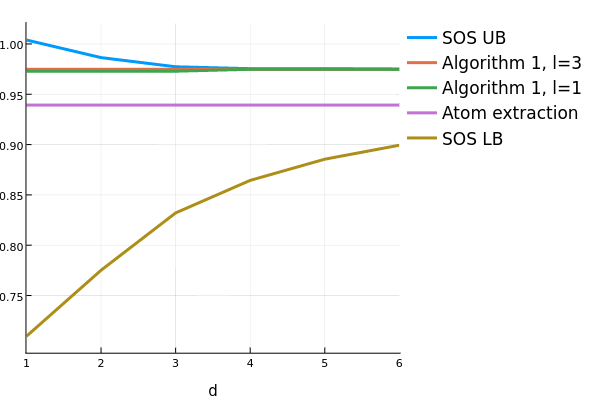
\includegraphics[width=\textwidth]{../../latex/images/PEDJ.png}
  \end{subfigure}
  \begin{subfigure}{0.48\textwidth}
    \centering
    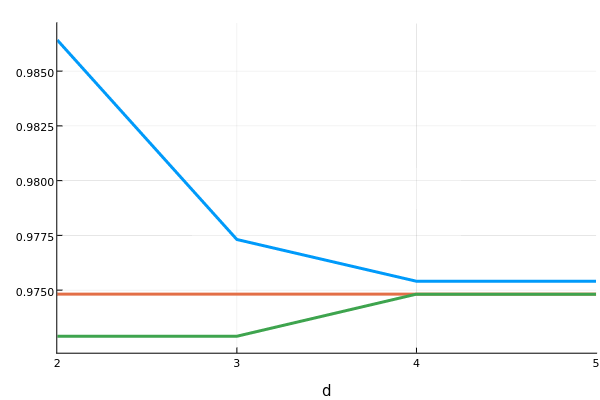
\includegraphics[width=\textwidth]{../../latex/images/PEDJ_zoom.png}
  \end{subfigure}
  \caption{Result of \exemref{run4}. The SOS UB is the upper bound found by \progref{primal} and the SOS LB is obtained from this upper bound the guarantee given in \cororef{mix}. The value $d$ of horizontal axis corresponds to using polynomials of degree $2d$. The right figure is a zoom of the left figure.}
  \label{fig:pedj}
\end{figure}

